\documentclass{bmvc2k}

%% Paper ID placeholder — replace with assigned ID upon OpenReview registration
\bmvcreviewcopy{??}

\title{Why Deep ResNets Train Successfully:\\
Self-Selection of Effective Depth Enabled by Skip Connections}

% Anonymized for double-blind review
\addauthor{Anonymous}{}{1}

\addinstitution{
 Anonymous Institution\\
 Anonymous Address
}

\runninghead{Anonymous}{Self-Selection of Effective Depth in ResNets}

% Macros
\def\eg{\emph{e.g}\bmvaOneDot}
\def\Eg{\emph{E.g}\bmvaOneDot}
\def\etal{\emph{et al}\bmvaOneDot}

\usepackage{amssymb}
\usepackage{amsmath}
\usepackage{booktabs}
\usepackage{multirow}
\usepackage{xcolor}
\usepackage{subcaption}
\usepackage{hyperref}

%-------------------------------------------------------------------------
\begin{document}

\maketitle

\begin{abstract}
A decade after their introduction, the precise mechanism behind the success of deep Residual Networks (ResNets) remains debated. Why does adding more layers \emph{not} degrade performance, when plain networks of the same depth fail catastrophically? We propose an explanation grounded in direct measurement: \textbf{deep ResNets succeed because they autonomously select an effective depth far smaller than their nominal depth, and skip connections are the mechanism that enables this self-selection.}
To make this self-selection \emph{directly observable}, we introduce \textbf{Learnable Residual Scaling (LRS)}, an analytical instrument that attaches a single learnable scalar $\alpha$ to each residual block: $y = \alpha \cdot F(x) + (1 - \alpha) \cdot x$ with $\alpha = \sigma(\theta) \in (0,1)$. Because the two coefficients sum to one, the learned $\alpha_i$ directly reports block $i$'s usage---no post-hoc analysis required.
Three lines of evidence support our thesis. \emph{(i) Plain networks cannot self-select and fail}: without skip connections, gradient norms at initialization explode to $10^{13}$ in early blocks. \emph{(ii) ResNets autonomously compress effective depth}: across CIFAR-10/100 and ImageNet (depths 50--200), the mean $\bar{\alpha}$ decreases monotonically with depth (e.g., $0.34 \to 0.11$ as depth grows $50 \to 200$ on CIFAR-100); per-block analysis shows only 5--6 of 66 blocks remain active in a 200-layer network. \emph{(iii) The selection is intrinsic}: identity vs random initialization converge to nearly identical $\bar{\alpha}$, and $\alpha$-guided pruning validates the measurement---blocks with $\alpha < 0.03$ can be removed with \emph{zero} accuracy loss, and pruning $56\%$ of blocks reduces FLOPs by $54\%$ and latency by $52\%$ at only $4.6\%$ accuracy cost.
The depth--$\alpha$ scaling law generalizes to ImageNet, where ResNet-50/101 produce $\bar{\alpha}$ values matching their CIFAR counterparts. This reframes the degradation problem: it is not failure to be solved, but the network correctly refusing to use redundant depth.
\end{abstract}

%-------------------------------------------------------------------------
\section{Introduction}
\label{sec:intro}

Residual Networks (ResNets)~\cite{he2016deep} enable the training of networks with hundreds of layers, while plain networks of comparable depth fail catastrophically. The standard explanation---``skip connections stabilize gradient flow''---is technically correct but mechanistically incomplete. Skip connections do stabilize gradients, but this alone does not explain \emph{why deeper ResNets do not degrade}. If skip connections merely allow more computation, deeper networks should be at least as expressive as shallower ones; in practice they are, but only because of \emph{how} that capacity is used. The question we address is the next one: \textbf{what does the network do with the depth that skip connections make available to it?}

We propose a concrete answer: \emph{deep ResNets train successfully because they autonomously select an effective depth far smaller than their nominal depth, and skip connections are the architectural mechanism that enables this self-selection.} Adding nominal depth does not commit the network to using all of it---skip connections provide the freedom to refuse. The degradation problem of plain networks is thus not solved by skip connections in the sense of ``making all layers trainable''; it is sidestepped by giving the network the option to \emph{choose how deep to be}.

Demonstrating this thesis requires a measurement tool: we need to read off, per block, how much the network actually uses that block. Existing residual scaling methods---ReZero~\cite{bachlechner2021rezero}, SkipInit~\cite{de2020batch}, Fixup~\cite{zhang2019fixup}, LayerScale~\cite{touvron2021going}---scale only $F(x)$ while leaving the identity at weight $1$, which is sufficient for stabilizing training but does not yield a per-block usage scalar. Veit \etal~\cite{veit2016residual} inferred shorter-than-nominal effective paths via path-counting and lesion studies, but their evidence is indirect.

\textbf{Learnable Residual Scaling (LRS).} We introduce a minimal modification to the residual block:
\begin{equation}
y = \alpha \cdot F(x) + (1-\alpha) \cdot x, \qquad \alpha = \sigma(\theta) \in (0,1),
\label{eq:lrs}
\end{equation}
where $\theta$ is a single learnable scalar per block. Because the two coefficients sum to one, the learned $\alpha_i$ \emph{is} block $i$'s usage: $\alpha_i \to 0$ means the block is effectively an identity (bypassed), $\alpha_i \to 1$ means a full transformation. LRS is not a performance method---it is a measurement instrument. Per-block scalars make depth self-selection \emph{directly observable} rather than inferred.

\textbf{Three lines of evidence.} We support the self-selection thesis with empirical evidence organized around three claims.

\emph{(a) Plain networks cannot self-select, hence they fail.} Figure~\ref{fig:gradient_flow} shows per-block gradient L2 norms at initialization for a 200-layer network on CIFAR-100. Without skip connections, the gradient at Block 0 reaches $1.72 \times 10^{13}$ while Block 65 sits at $5.0$---a $3.5 \times 10^{12}\times$ disparity that makes meaningful learning impossible. Skip connections stabilize this disparity to $673\times$, but our LRS measurements (panels b--c) reveal that the network does not use this stability to leverage all blocks. Instead, gradients in late blocks decay to near zero, reflecting learned $\alpha_i \approx 0$: the network is not attempting to train those blocks at all.

\emph{(b) ResNets autonomously compress effective depth.} Across four depths ($50, 101, 152, 200$), two CIFAR datasets, and ImageNet at depths $50$ and $101$ (three seeds each for CIFAR), the mean converged $\bar{\alpha}$ decreases systematically with depth (e.g., $0.34 \to 0.11$ as depth grows $50 \to 200$ on CIFAR-100). Per-block analysis shows only 5--6 of 66 blocks maintain $\alpha > 0.3$ in a 200-layer network. The threshold-free metric $D_\text{eff} = \sum_i \alpha_i$ confirms that quadrupling blocks ($16 \to 66$) increases effective depth by only $40\%$ ($5.4 \to 7.5$). The network is given depth and chooses to ignore most of it.

\emph{(c) The selection is intrinsic, not an artifact.} Three controls argue against optimization-induced bias. First, identity initialization of the residual branch yields nearly identical converged $\bar{\alpha}$ ($0.114$ vs.\ $0.118$ for random init), showing the result does not depend on the starting point. Second, $\alpha$-guided block pruning validates the measurement: blocks with $\alpha < 0.03$ can be removed without retraining and incur \emph{zero} accuracy loss; pruning $56\%$ of blocks ($\alpha < 0.08$) followed by 10 epochs of fine-tuning recovers $75.91\%$ from the original $80.54\%$ while reducing FLOPs by $54\%$ and inference latency by $52\%$. Third, residual-favoring initialization ($\alpha_0 \approx 0.88$) causes catastrophic training failure at depth 200 (CIFAR-100: $37.50\pm29.20\%$), confirming that the identity-favored regime is not optional but necessary.

\begin{figure}[t]
    \centering
    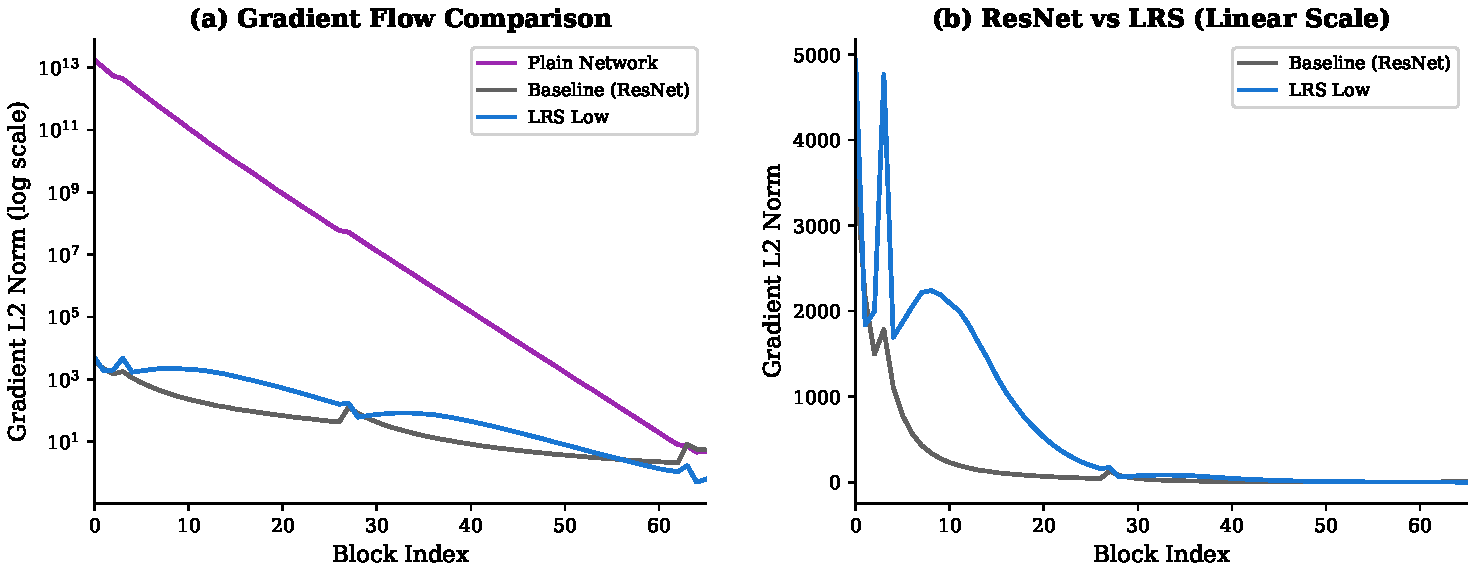
\includegraphics[width=\linewidth]{figures/fig0_gradient_flow.pdf}
    \caption{Per-block gradient L2 norms at initialization for ResNet-200 on CIFAR-100. (a) Plain networks without skip connections cannot self-select depth---gradients explode to $>10^{13}$ in early blocks. Skip connections stabilize the gradient distribution. (b--c) With LRS, late-block gradients decay toward zero, reflecting the network's learned choice $\alpha_i \approx 0$: those blocks are not used.}
    \label{fig:gradient_flow}
\end{figure}

\textbf{Contributions.}
(1) We propose that ResNets train successfully because of self-selection of effective depth, made possible by skip connections; LRS makes this measurable.
(2) We empirically establish a depth--$\alpha$ scaling law that holds across CIFAR-10/100 and ImageNet at multiple depths.
(3) We validate that the measurement is semantically meaningful through pruning, identity-init invariance, and initialization sensitivity analyses; $\alpha$-guided pruning achieves $54\%$ FLOPs reduction with $4.6\%$ accuracy cost.
(4) We reframe the degradation problem: it is not failure to be solved, but the network refusing to use depth it does not need.

%-------------------------------------------------------------------------
\section{Related Work}
\label{sec:related}

\subsection{Residual Networks and Skip Connections}

ResNet~\cite{he2016deep} introduced skip connections to alleviate gradient vanishing in deep networks. He \etal~\cite{he2016identity} further showed that identity mappings improve gradient flow. Highway Networks~\cite{srivastava2015highway} proposed gated information flow prior to ResNet, but ResNet's simpler additive shortcut proved more effective in practice. De \& Smith~\cite{de2020batch} showed that batch normalization biases standard ResNet residuals toward identity, a phenomenon LRS makes explicit but does not create.

\subsection{Residual Scaling Methods}

Several methods scale the residual branch (Table~\ref{tab:comparison}). \textbf{ReZero}~\cite{bachlechner2021rezero} initializes a scalar multiplier $\alpha = 0$ on the residual branch: $y = x + \alpha F(x)$. \textbf{SkipInit}~\cite{de2020batch} applies the same form with batch normalization retained. \textbf{Fixup}~\cite{zhang2019fixup} initializes the last BN of each block to zero so $F(x) \approx 0$ at start. \textbf{LayerScale}~\cite{touvron2021going} introduces per-channel learnable scaling in Vision Transformers. All these methods scale only $F(x)$ while keeping $x$ at weight $1$. LRS instead learns the relative weight of both branches via a single scalar, which is the key to per-block usage measurement.

\begin{table}[t]
\centering
\small
\caption{Residual scaling methods. Only LRS measures the relative ratio between $F(x)$ and $x$ as a single per-block scalar, enabling direct effective-depth measurement.}
\label{tab:comparison}
\begin{tabular}{lccc}
\toprule
\textbf{Method} & \textbf{Formulation} & \textbf{Per-block measurable} & \textbf{Key difference} \\
\midrule
ReZero & $y = x + \alpha F(x)$ & $|F(x)|$ scale & $x$ weight fixed at $1$ \\
SkipInit & $y = x + \alpha F(x)$ & $|F(x)|$ scale & $x$ weight fixed at $1$ \\
LayerScale & $y = x + \Lambda F(x)$ & per-channel $|F(x)|$ & $x$ weight fixed at $1$ \\
Fixup & $y = x + \beta F(x)$ & $|F(x)|$ scale & zero-init last layer \\
\textbf{LRS (ours)} & $\mathbf{y = \alpha F(x) + (1{-}\alpha)x}$ & $\mathbf{F(x){:}x}$ \textbf{ratio} & \textbf{both sides adjusted} \\
\bottomrule
\end{tabular}
\end{table}

\subsection{Comparison with Highway Networks}

Highway Networks~\cite{srivastava2015highway} use a similar-looking convex combination $y = T(x) F(x) + (1{-}T(x)) x$ with $T(x) = \sigma(W_g x + b_g)$. The distinction is structural and central to our analysis. Highway's transform gate $T(x)$ is \emph{input-dependent}: every input produces a different gate value, so per-block usage cannot be summarized by a single number. LRS instead uses an \emph{input-independent scalar} $\alpha = \sigma(\theta)$, deliberately removing input dependency to obtain a per-block measurement. This is a methodological choice for interpretability: a single $\alpha$ per block makes ``how much does this block transform its input'' a well-defined quantity, enabling the depth--$\alpha$ scaling law, the per-block distribution analysis, and the pruning validation that follow. Highway gates, by contrast, would require aggregating over input distributions to produce a comparable scalar---losing the very interpretability that motivates our design.

\subsection{Effective Depth and Network Redundancy}

Huang \etal~\cite{huang2016deep} proposed stochastic depth, randomly dropping residual blocks during training, showing that not all blocks are needed. The lottery ticket hypothesis~\cite{frankle2019lottery} demonstrated that large networks contain small subnetworks matching the full network's performance. The closest prior work is Veit \etal~\cite{veit2016residual}, which interpreted ResNets as ensembles of paths and showed empirically that effective paths are much shorter than nominal depth. However, prior evidence is \emph{indirect}: path-ensemble analysis counts paths of various lengths, and lesion studies infer importance by deleting blocks and measuring degradation. The question ``how much does block $i$ actually contribute'' is answered only inferentially. LRS provides a \emph{direct, per-block, quantitative measurement}: the learned $\alpha_i$ values are themselves the blocks' contributions, observable without any post-hoc analysis. This direct measurability enables (i) a quantitative scaling law $\bar{\alpha}(L)$, (ii) a threshold-free effective-depth metric $D_\text{eff} = \sum_i \alpha_i$, and (iii) a principled pruning criterion validated by zero-loss removal at $\alpha < 0.03$.

\subsection{Comparison with Trained-Importance Pruning}

A related line of work uses learnable scalars within blocks as importance signals for pruning. Network Slimming~\cite{liu2017slimming} repurposes Batch Normalization's $\gamma$ as a per-channel importance score, applying $L_1$ regularization to induce sparsity. The mechanism is superficially similar---a learned scalar reveals component usage---but the operand and semantic differ fundamentally on three axes. \textbf{Granularity}: Network Slimming measures \emph{per-channel} importance within a fixed depth; LRS measures \emph{per-block} usage and yields a network-level effective depth $D_\text{eff}$. \textbf{Interpretation}: $\gamma$ scales a single normalized feature and requires explicit $L_1$ pressure to become sparse; $\alpha$ is a convex-combination weight whose semantics (the $F{:}x$ ratio) are intrinsic---no sparsity prior is applied, and small $\alpha$ emerges from training dynamics alone. \textbf{Claim}: Network Slimming is a pruning method; LRS is an analytical instrument whose pruning experiment is a \emph{validation} of the self-selection thesis, not the contribution itself. Channel Pruning~\cite{he2017channel} and similar trained-importance methods share Network Slimming's perspective and are likewise complementary to ours.

%-------------------------------------------------------------------------
\section{Method}
\label{sec:method}

\subsection{Learnable Residual Scaling}

We redefine the residual block (Eq.~\ref{eq:lrs}) where $\theta$ is a learnable scalar parameter per block and $\sigma$ is the sigmoid. The parameterization serves two purposes. First, since $\alpha + (1-\alpha) = 1$, the \emph{relative ratio} between $F(x)$ and $x$ is directly interpretable: $\alpha = 0.14$ means the block allocates $14\%$ weight to the transformation and $86\%$ to the identity. Second, the bounded range ensures numerical stability. The semantics give a natural definition of effective depth: $\alpha \to 0$ means the block is effectively bypassed ($y \approx x$); $\alpha \to 1$ means a full transformation. The effective depth of the network is the number of blocks with $\alpha$ above a meaningful threshold, with $D_\text{eff} = \sum_i \alpha_i$ as a threshold-free analogue.

\subsection{Gradient Flow Analysis}

The backward pass through an LRS block yields:
\begin{equation}
    \frac{\partial \mathcal{L}}{\partial x} = \frac{\partial \mathcal{L}}{\partial y} \left[ (1 - \alpha) + \alpha \cdot F'(x) \right]
    \label{eq:grad}
\end{equation}
and the total gradient through $L$ blocks is the product:
\begin{equation}
    \frac{\partial \mathcal{L}}{\partial x_0} = \frac{\partial \mathcal{L}}{\partial y_L} \cdot \prod_{i=1}^{L} \left[ (1 - \alpha_i) + \alpha_i \cdot F'_i(x_i) \right].
    \label{eq:total_grad}
\end{equation}
This product structure explains the depth--$\alpha$ relationship. For the product to remain stable across $L$ blocks, each factor must be close to $1$. When $\alpha_i$ is small, the factor approaches $(1{-}\alpha_i) \approx 1$ regardless of $F'_i$, ensuring gradient stability. As $L$ grows, smaller $\alpha_i$ values are needed to maintain the product near unity, providing a theoretical basis for why deeper networks should converge to smaller $\bar{\alpha}$. Conversely, when $\alpha_i$ is large, the factor becomes $\approx F'_i$ and the gradient product degenerates to that of a plain network, prone to vanishing or explosion. This predicts that residual-favoring initialization leads to training collapse at extreme depth---verified in Section~\ref{sec:init_sensitivity}.

\subsection{Initialization Variants}

We test three initialization strategies (Table~\ref{tab:init_variants}) to study convergence and sensitivity. These serve as probes: if the optimization landscape has a single basin, all three converge to the same $\bar{\alpha}$; otherwise, divergence reveals the role of initial conditions.

\begin{table}[t]
\centering
\small
\caption{LRS variants by $\alpha$ initialization. The three starting points probe whether $\alpha$ converges to the same optimum.}
\label{tab:init_variants}
\begin{tabular}{lccc}
\toprule
\textbf{Variant} & $\theta_0$ & $\alpha_0$ & \textbf{Initial bias} \\
\midrule
LRS Low  & $-2.0$ & $\approx 0.12$ & identity-favoring \\
LRS Mid  & $0.0$  & $0.50$         & balanced \\
LRS High & $+2.0$ & $\approx 0.88$ & residual-favoring \\
\bottomrule
\end{tabular}
\end{table}

%-------------------------------------------------------------------------
\section{Experiments}
\label{sec:experiments}

\subsection{Experimental Setup}
\label{sec:setup}

\textbf{Datasets.} CIFAR-10/100~\cite{krizhevsky2009learning} (10/100 classes, 50K/10K train/test) for systematic analysis; ImageNet~\cite{russakovsky2015imagenet} (1000 classes, 1.28M/50K) for scale validation.

\textbf{Architectures.} Bottleneck ResNet-50/101/152/200 (16/33/50/66 blocks). CIFAR uses a $3{\times}3$ stride-1 stem; ImageNet uses the standard $7{\times}7$ stride-2 + max-pool stem~\cite{he2016deep}.

\textbf{Training.} CIFAR: SGD with momentum 0.9, weight decay $10^{-4}$; initial LR $0.1$ with cosine annealing~\cite{loshchilov2017sgdr}; 5-epoch linear warmup; 100 epochs. Batch size is depth-dependent due to GPU memory ($128, 64, 32, 32$ at depths $50, 101, 152, 200$). ImageNet: same optimizer, LR $0.2$, batch size $512$ (fixed), $60$ epochs, $5$-epoch warmup. All CIFAR experiments use 3 seeds (42, 123, 456) and report mean $\pm$ std; ImageNet uses a single seed due to compute. The batch-size variation across CIFAR depths is a known confound; however, ImageNet at \emph{fixed} batch size $512$ shows the same $\bar{\alpha}$ scaling slope ($d50 \to d101$: $0.303 \to 0.166$, $45\%$ drop) as CIFAR-100 with variable batch sizes ($0.342 \to 0.183$, $46\%$ drop), arguing that batch size is not the driver of the depth--$\bar{\alpha}$ relationship.

\textbf{Models.} Five core variants: Baseline (standard ResNet), LRS Low/Mid/High ($\alpha_0 \in \{0.12, 0.5, 0.88\}$), and ReZero. For method comparison we additionally evaluate SkipInit, Fixup, and LayerScale.

\subsection{Depth--$\alpha$ Scaling Law}
\label{sec:alpha_convergence}

We first measure the central observation: how does the network's preferred $\bar{\alpha}$ change with depth? Table~\ref{tab:depth_alpha} reports converged $\bar{\alpha}$ on CIFAR-100 across the three initialization variants (3-seed mean).

\begin{table}[t]
\centering
\small
\caption{Mean converged $\bar{\alpha}$ by depth on CIFAR-100 (3-seed average). Low and Mid converge to similar final values; High diverges at extreme depth.}
\label{tab:depth_alpha}
\begin{tabular}{lcccc}
\toprule
\textbf{Depth} & \textbf{Blocks} & \textbf{LRS Low} & \textbf{LRS Mid} & \textbf{LRS High} \\
\midrule
50  & 16 & 0.34 & 0.35 & 0.36 \\
101 & 33 & 0.18 & 0.20 & 0.21 \\
152 & 50 & 0.13 & 0.15 & 0.23 \\
200 & 66 & 0.11 & 0.13 & 0.28 \\
\bottomrule
\end{tabular}
\end{table}

Several observations emerge. (i) \textbf{Monotonic decrease with depth.} The converged $\bar{\alpha}$ decreases from $0.34$ (depth 50) to $0.11$ (depth 200) for LRS Low---each block's contribution shrinks as more blocks are added. (ii) \textbf{Partial convergence across initializations.} At depth 50, all three variants converge to similar values ($0.34$--$0.36$). At depth 200, the High variant settles at $0.28$, significantly above the $0.11$--$0.13$ range of Low/Mid, with severely degraded performance (Section~\ref{sec:init_sensitivity}). (iii) \textbf{Dataset independence.} CIFAR-10 yields nearly identical $\bar{\alpha}$ at each depth, suggesting an architectural rather than data-driven property.

\textbf{Verification at scale.} To confirm the law generalizes beyond CIFAR, we measure $\bar{\alpha}$ on ImageNet at two depths (Figure~\ref{fig:depth_alpha}). ResNet-50 yields $\bar{\alpha} = 0.303$, ResNet-101 yields $\bar{\alpha} = 0.166$. Both values closely track their CIFAR-100 counterparts ($0.342, 0.183$) and follow the same scaling trend. ImageNet has $\sim$25$\times$ more training samples, 10$\times$ more classes, and 7$\times$ larger input resolution than CIFAR; the persistence of the $\alpha$ pattern across this gap rules out simple dataset-size explanations.

Although ImageNet uses a single seed due to compute, the CIFAR scaling law has tight cross-seed variance: $\bar{\alpha}$ std at depths $(50, 101, 152, 200)$ is $(0.0007, 0.0005, 0.0012, 0.0002)$---all below $1\%$ of the mean. The ImageNet--CIFAR-100 gaps at matched depths are $0.342{-}0.303 = 0.039$ at $d50$ and $0.183{-}0.166 = 0.017$ at $d101$, both 20--80$\times$ larger than the CIFAR seed-noise scale, indicating a small but systematic dataset shift while preserving monotonicity. The ratio of ImageNet $\bar{\alpha}$ at $d50 \to d101$ is $0.303/0.166 = 1.83$, essentially matching the CIFAR-100 ratio $0.342/0.183 = 1.87$; the scaling law's slope is preserved across the dataset gap. A statistical accident producing the same decreasing trend across two depths at this gap-to-noise ratio is implausible.

\begin{figure}[t]
    \centering
    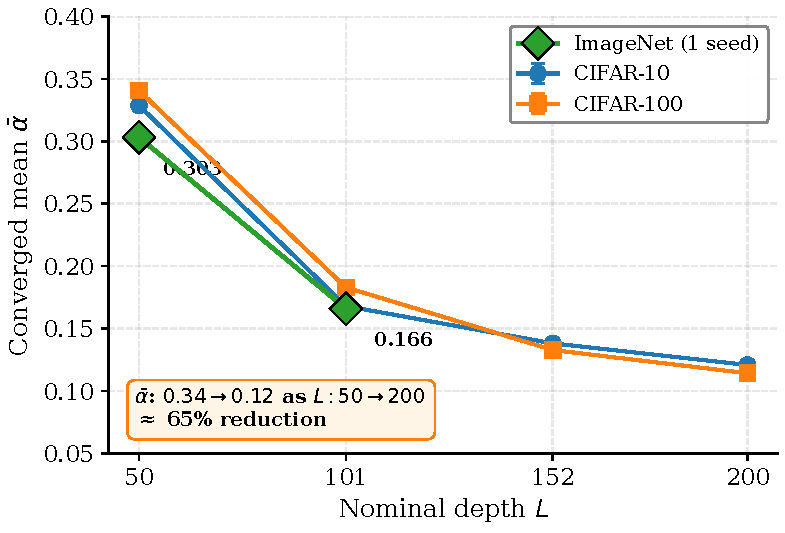
\includegraphics[width=0.85\linewidth]{figures/fig_depth_alpha_v2.pdf}
    \caption{The depth--$\bar{\alpha}$ scaling law. Mean converged $\bar{\alpha}$ decreases monotonically with nominal depth $L$ across CIFAR-10, CIFAR-100, and ImageNet. As depth grows $50 \to 200$, ResNets autonomously suppress $\sim$65\% of their residual contribution. Error bars: $\pm 1$ std over 3 seeds (CIFAR); ImageNet uses a single seed.}
    \label{fig:depth_alpha}
\end{figure}

\subsection{Per-Block $\alpha$ Distribution}
\label{sec:perblock}

The mean hides structure. Figure~\ref{fig:perblock_alpha} shows per-block $\alpha$ for a 200-layer network (66 blocks, LRS Low, CIFAR-100). Two patterns emerge: \textbf{downsampling blocks have high $\alpha$} (0.42--0.96), and \textbf{normal blocks have low $\alpha$} (0.06--0.15) with progressive decrease toward stage end. The network treats each stage as ``one essential transformation (downsampling) followed by progressively negligible refinements.''

\begin{figure}[t]
    \centering
    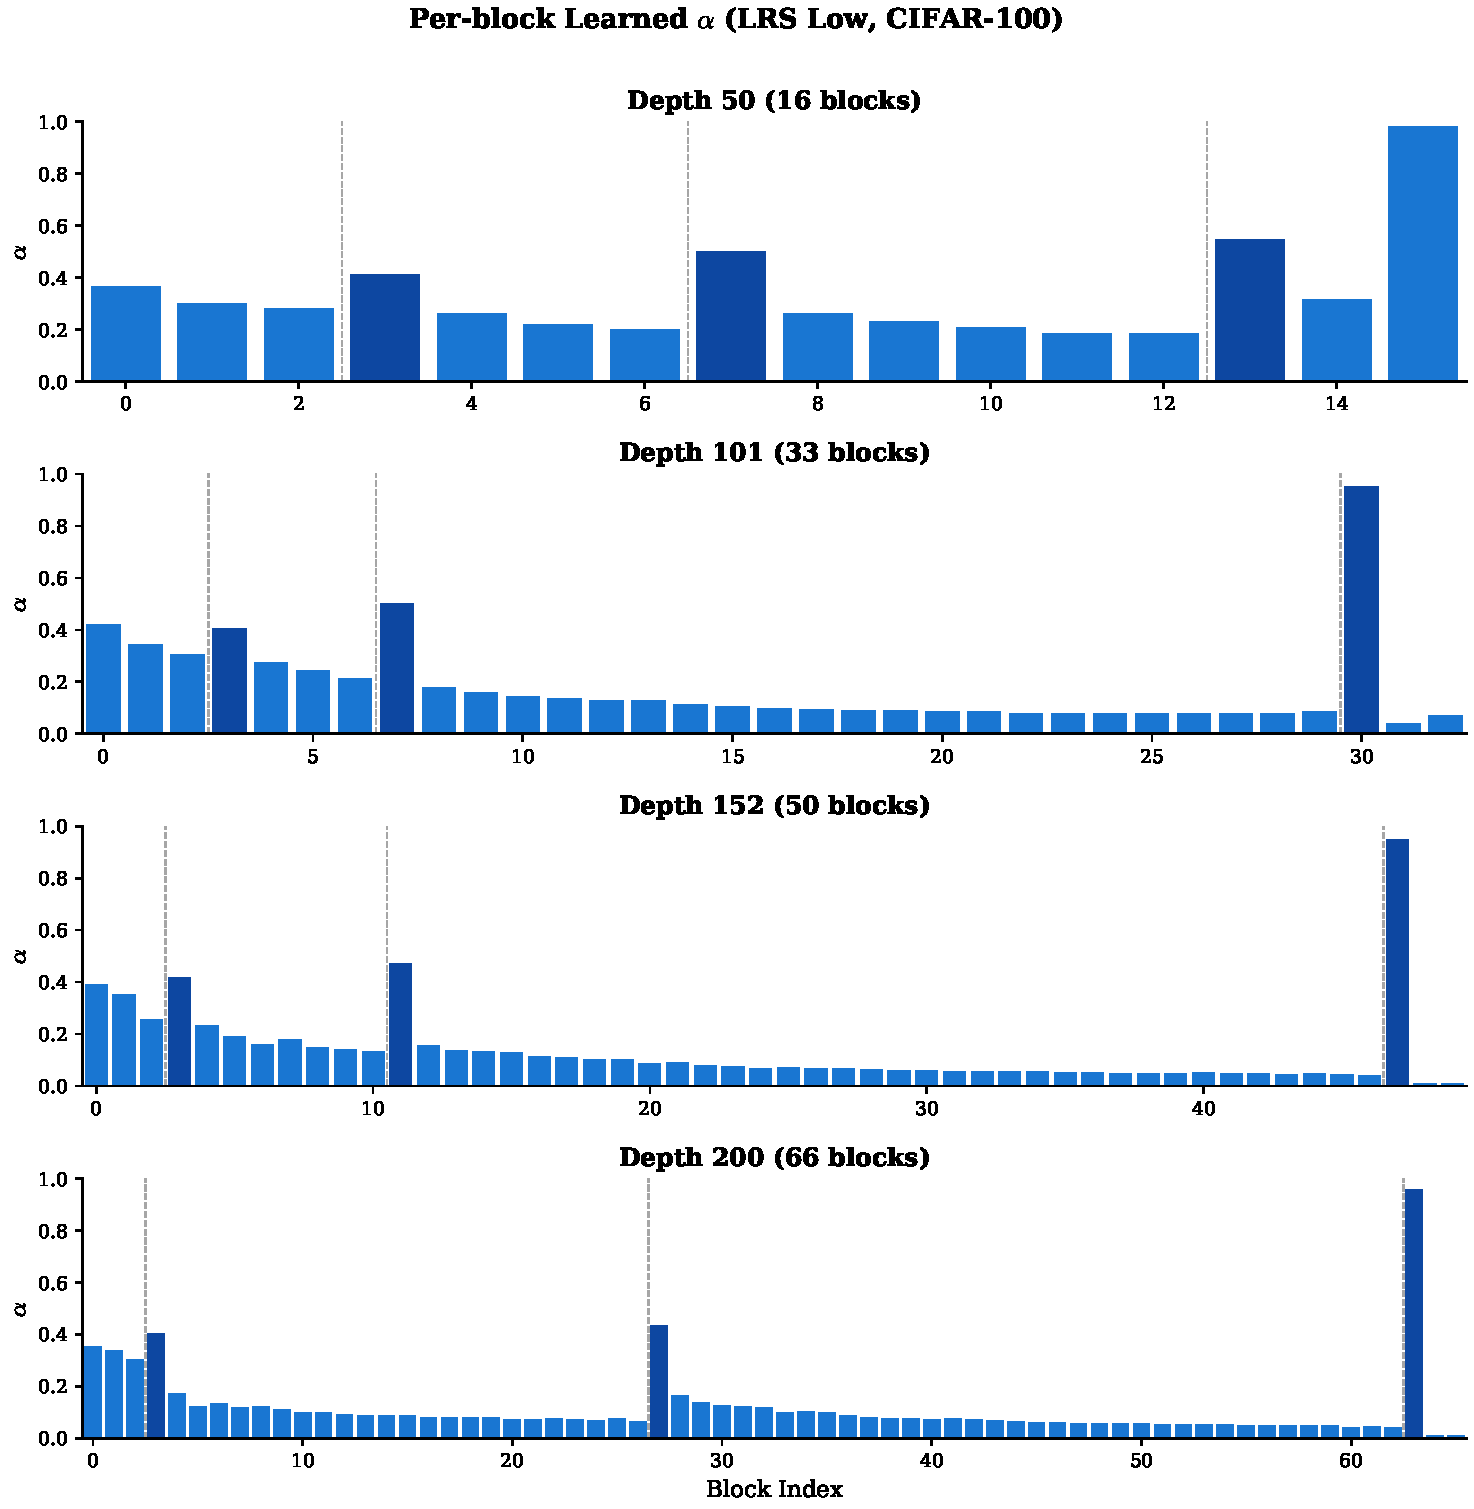
\includegraphics[width=\linewidth]{figures/fig4_perblock_alpha.pdf}
    \caption{Per-block $\alpha$ for ResNet-200 on CIFAR-100. Stage boundaries (downsampling blocks) maintain high $\alpha$; within-stage blocks converge to near-zero values.}
    \label{fig:perblock_alpha}
\end{figure}

\subsection{Effective Depth Quantification}
\label{sec:effective_depth}

Using $\alpha > 0.3$ as ``active block'' threshold (Table~\ref{tab:effective_depth}), only 5--6 of 66 blocks in a 200-layer network qualify---effective depth $\sim$8\% of nominal. To avoid threshold dependence, we additionally report $D_\text{eff} = \sum_i \alpha_i$ (Table~\ref{tab:deff}): quadrupling blocks ($16 \to 66$) increases $D_\text{eff}$ by only $40\%$ ($5.4 \to 7.5$).

\begin{table}[t]
\centering
\small
\caption{Effective depth at ResNet-200/CIFAR-100, LRS Low.}
\label{tab:effective_depth}
\begin{tabular}{lcc}
\toprule
\textbf{Metric} & \textbf{Value} & \textbf{Interpretation} \\
\midrule
Nominal blocks & 66 & total residual blocks \\
Active blocks ($\alpha > 0.3$) & 5--6 & meaningfully transforming \\
Effective depth ratio & $\sim$8\% & fraction of blocks used \\
$\bar{\alpha}$ (normal blocks) & 0.06--0.15 & near-identity \\
$\bar{\alpha}$ (downsampling blocks) & 0.42--0.96 & active transformation \\
\bottomrule
\end{tabular}
\end{table}

\begin{table}[t]
\centering
\small
\caption{Threshold-free effective depth $D_\text{eff} = \sum_i \alpha_i$ for LRS Low on CIFAR-100. Although nominal depth scales 4$\times$, $D_\text{eff}$ scales only 1.4$\times$.}
\label{tab:deff}
\begin{tabular}{lccc}
\toprule
\textbf{Depth} & \textbf{Blocks} ($N$) & $D_\text{eff} = \sum \alpha_i$ & $D_\text{eff}/N$ \\
\midrule
50  & 16 & 5.4 & 34.0\% \\
101 & 33 & 6.0 & 18.3\% \\
152 & 50 & 6.7 & 13.3\% \\
200 & 66 & 7.5 & 11.4\% \\
\bottomrule
\end{tabular}
\end{table}

\subsection{Initialization Sensitivity}
\label{sec:init_sensitivity}

The three initializations reveal dramatic differences in training stability with depth (Tables~\ref{tab:cifar10}, \ref{tab:cifar100}). LRS Low matches or beats baseline at all depths with low variance. LRS Mid degrades at depth 200. LRS High shows progressive degradation, culminating in catastrophic failure (CIFAR-100: $37.50 \pm 29.20\%$). The mechanism is gradient-preservation (Eq.~\ref{eq:total_grad}): with $\alpha_0 = 0.88$, the identity baseline is $0.12^{66} \approx 0$ through 66 blocks, making learning impossible without rapid $\alpha$ adjustment---which itself requires gradients.

\begin{table}[t]
\centering
\small
\caption{CIFAR-10 test accuracy (\%, 3-seed mean $\pm$ std). LRS High collapses at depth 200.}
\label{tab:cifar10}
\begin{tabular}{lccccc}
\toprule
\textbf{Depth} & \textbf{Baseline} & \textbf{LRS Low} & \textbf{LRS Mid} & \textbf{LRS High} & \textbf{ReZero} \\
\midrule
50  & 94.53$\pm$0.14 & \textbf{94.83}$\pm$0.13 & 94.77$\pm$0.03 & 94.27$\pm$0.17 & 94.60$\pm$0.28 \\
101 & 95.37$\pm$0.11 & \textbf{95.44}$\pm$0.12 & 95.15$\pm$0.11 & 94.28$\pm$0.29 & 95.38$\pm$0.21 \\
152 & 95.95$\pm$0.06 & 95.73$\pm$0.10 & 95.60$\pm$0.15 & 93.78$\pm$0.87 & \textbf{95.99}$\pm$0.06 \\
200 & 95.98$\pm$0.15 & \textbf{96.10}$\pm$0.12 & 94.36$\pm$0.92 & 67.25$\pm$43.65 & 96.02$\pm$0.16 \\
\bottomrule
\end{tabular}
\end{table}

\begin{table}[t]
\centering
\small
\caption{CIFAR-100 test accuracy (\%, 3-seed mean $\pm$ std). LRS High fails catastrophically.}
\label{tab:cifar100}
\begin{tabular}{lccccc}
\toprule
\textbf{Depth} & \textbf{Baseline} & \textbf{LRS Low} & \textbf{LRS Mid} & \textbf{LRS High} & \textbf{ReZero} \\
\midrule
50  & 77.18$\pm$0.36 & 77.02$\pm$0.20 & 76.72$\pm$0.40 & 75.22$\pm$0.45 & 76.12$\pm$0.09 \\
101 & \textbf{79.29}$\pm$0.23 & 78.85$\pm$0.14 & 78.34$\pm$0.19 & 75.16$\pm$1.69 & 78.04$\pm$0.48 \\
152 & \textbf{80.42}$\pm$0.22 & 80.28$\pm$0.38 & 78.57$\pm$0.60 & 71.66$\pm$3.40 & 79.72$\pm$0.10 \\
200 & \textbf{80.72}$\pm$0.17 & 80.65$\pm$0.01 & 76.07$\pm$1.59 & 37.50$\pm$29.20 & 80.14$\pm$0.17 \\
\bottomrule
\end{tabular}
\end{table}

\subsection{Intrinsic vs.\ Artifact: Identity Initialization Test}
\label{sec:identity_init}

A natural concern: is the low effective depth an artifact of randomly initialized residual branches? We test this by initializing residual branches as identity transformations (HybridA: identity init for layers 3 \& 4; Full Identity: all layers). Results on CIFAR-100 (Table~\ref{tab:identity_init}): full identity init catastrophically fails (12.98\% at depth 200) due to symmetry that the network cannot break. Partial identity + LRS achieves the best accuracy (81.14\%). \emph{Crucially}, the learned $\bar{\alpha}$ is nearly identical between random and identity init ($0.114$ vs.\ $0.118$, with 5 vs.\ 6 active blocks out of 66). The network converges to the same effective depth regardless of where the residual branch starts---ruling out initialization as the source of low effective depth.

\begin{table}[t]
\centering
\small
\caption{Identity init analysis (CIFAR-100, 3-seed mean $\pm$ std). Effective depth is invariant to residual branch initialization.}
\label{tab:identity_init}
\begin{tabular}{lcccc}
\toprule
\textbf{Model} & \textbf{d152 (\%)} & \textbf{d200 (\%)} & $\mathbf{\bar{\alpha}}$ \textbf{(d200)} & \textbf{Active / 66} \\
\midrule
Baseline (He init) & 80.42$\pm$0.18 & 80.72$\pm$0.13 & --- & --- \\
LRS Low + He init & 80.28$\pm$0.31 & 80.65$\pm$0.01 & 0.114 & 5 \\
HybridA (Identity L3,4) & 80.02$\pm$0.26 & 80.40$\pm$0.17 & --- & --- \\
LRS Low + HybridA & \textbf{80.72}$\pm$0.29 & \textbf{81.14}$\pm$0.18 & 0.118 & 6 \\
ResNet (Full Identity) & 13.41$\pm$0.41 & 12.98$\pm$0.16 & --- & --- \\
\bottomrule
\end{tabular}
\end{table}

\subsection{Fixed vs.\ Learned $\alpha$}
\label{sec:fixed_alpha}

To validate that \emph{learning} $\alpha$ is essential, we compare with fixed-$\alpha$ variants at depth 152 (Table~\ref{tab:fixed_alpha}). Two findings emerge. (i) Fixed $\alpha = 0.5$ yields only $44.19\%$ because the formulation $0.5 F(x) + 0.5 x$ halves both branches uniformly, unlike standard ResNet's $F(x) + x$. We include this point for completeness of the sweep; the resulting drop confounds the role of magnitude with the role of allocation and should not be read as the load-bearing comparison. (ii) The relevant comparison is fixed $\alpha = 0.1$, close to the learned mean, which still underperforms learned LRS by $0.47\%$. While modest, this gap is consistent with learned LRS exploiting per-block heterogeneity: downsampling blocks maintain $\alpha \in [0.42, 0.96]$ while within-stage blocks settle near $\alpha \in [0.06, 0.15]$ (Section~\ref{sec:perblock}). A uniform constant cannot capture this structure.

\begin{table}[t]
\centering
\small
\caption{Fixed vs.\ learned $\alpha$ at depth 152, CIFAR-100. Learned per-block structure is essential.}
\label{tab:fixed_alpha}
\begin{tabular}{lcc}
\toprule
\textbf{Configuration} & \textbf{Accuracy (\%)} & \textbf{Notes} \\
\midrule
Learned (LRS Low) & \textbf{80.28} & per-block $\alpha$, mean $\approx 0.13$ \\
Fixed $\alpha = 0.1$ & 79.81 & close to learned mean \\
Fixed $\alpha = 0.3$ & 67.94 & moderate transformation \\
Fixed $\alpha = 0.5$ & 44.19 & halves both branches \\
Fixed $\alpha = 0.7$ & 20.62 & residual-favoring \\
\midrule
Baseline ($F(x){+}x$) & 80.42 & no LRS \\
\bottomrule
\end{tabular}
\end{table}

\subsection{$\alpha$-Guided Pruning and Efficiency}
\label{sec:pruning}

If $\alpha_i$ truly reports block usage, then blocks with very low $\alpha$ should be removable without harm---a direct empirical test of our thesis. We prune blocks with $\alpha < \tau$ for various thresholds, replacing them with identity, and measure accuracy, FLOPs, and inference latency (NVIDIA A100 GPU, batch size 1).

Table~\ref{tab:pruning} reports the results on ResNet-200/CIFAR-100. Three findings:

\begin{table}[t]
\centering
\small
\caption{$\alpha$-guided pruning on ResNet-200/CIFAR-100. Accuracy retained through 10 epochs of fine-tuning; FLOPs and latency measured on actual short-circuited forward pass.}
\label{tab:pruning}
\begin{tabular}{lcccccc}
\toprule
\textbf{Threshold} & \textbf{Removed} & \textbf{Acc no-FT} & \textbf{Acc +FT} & $\mathbf{\Delta}$\textbf{Acc} & \textbf{FLOPs} & \textbf{Latency} \\
\midrule
None (orig.) & 0 / 66 & 80.54\% & --- & --- & 100.0\% & 100.0\% \\
$\alpha < 0.03$ & 2 / 66 & 80.54\% & \textbf{80.55\%} & \textbf{$+$0.01} & 97.1\% & 97.7\% \\
$\alpha < 0.05$ & 10 / 66 & 73.88\% & 79.65\% & $-$0.89 & 85.4\% & 86.1\% \\
$\alpha < 0.08$ & 37 / 66 & 3.97\% & 75.91\% & $-$4.63 & \textbf{45.8\%} & \textbf{48.5\%} \\
$\alpha < 0.10$ & 48 / 66 & 3.13\% & 74.74\% & $-$5.80 & 29.7\% & 32.3\% \\
$\alpha < 0.15$ & 58 / 66 & 3.63\% & 72.63\% & $-$7.91 & 15.0\% & 18.0\% \\
\bottomrule
\end{tabular}
\end{table}

\textbf{(a)~Zero-loss pruning at $\alpha < 0.03$.} Two blocks (12 conv/BN layers) can be removed \emph{without} retraining and \emph{without} accuracy loss. This is a direct semantic validation: blocks the network labels as $\alpha \approx 0$ truly contribute nothing.

\textbf{(b)~Practical efficiency gains.} At $\alpha < 0.08$, $56\%$ of blocks can be removed with $54\%$ FLOPs and $52\%$ latency reduction at a cost of $4.6\%$ accuracy after fine-tuning---a strong efficiency-accuracy trade-off. At $\alpha < 0.10$ (73\% pruned), the network retains $74.74\%$ accuracy with only $30\%$ of the original FLOPs.

\textbf{(c)~Self-selection vs.\ minimum sufficient depth.} Without fine-tuning, removing $\alpha < 0.08$ blocks collapses accuracy to $3.97\%$, but 10 epochs of fine-tuning recover it to $75.91\%$. At first glance this might appear to contradict the ``5--6 essential blocks'' claim. It does not. The $\alpha_i$ values measure each block's \emph{learned allocation under the original training}---they identify which blocks the network \emph{chose} to use, not which blocks are \emph{uniquely capable} of carrying that role. The 5--6 active blocks are essential \emph{conditional on the trained configuration}: removing them without fine-tuning collapses accuracy to $3.97\%$. The recovery via fine-tuning is a separate property of the network's \emph{capacity reserve}: 60 dormant blocks, each individually near-identity, can collectively re-learn the missing computation when forced to. Self-selection is thus a statement about \emph{learned} effective depth, not about \emph{minimum sufficient} depth---and the gap between them is precisely the ``reserve'' that skip connections preserve as latent capacity.

Figure~\ref{fig:pruning} visualizes the accuracy-efficiency trade-off.

\begin{figure}[t]
    \centering
    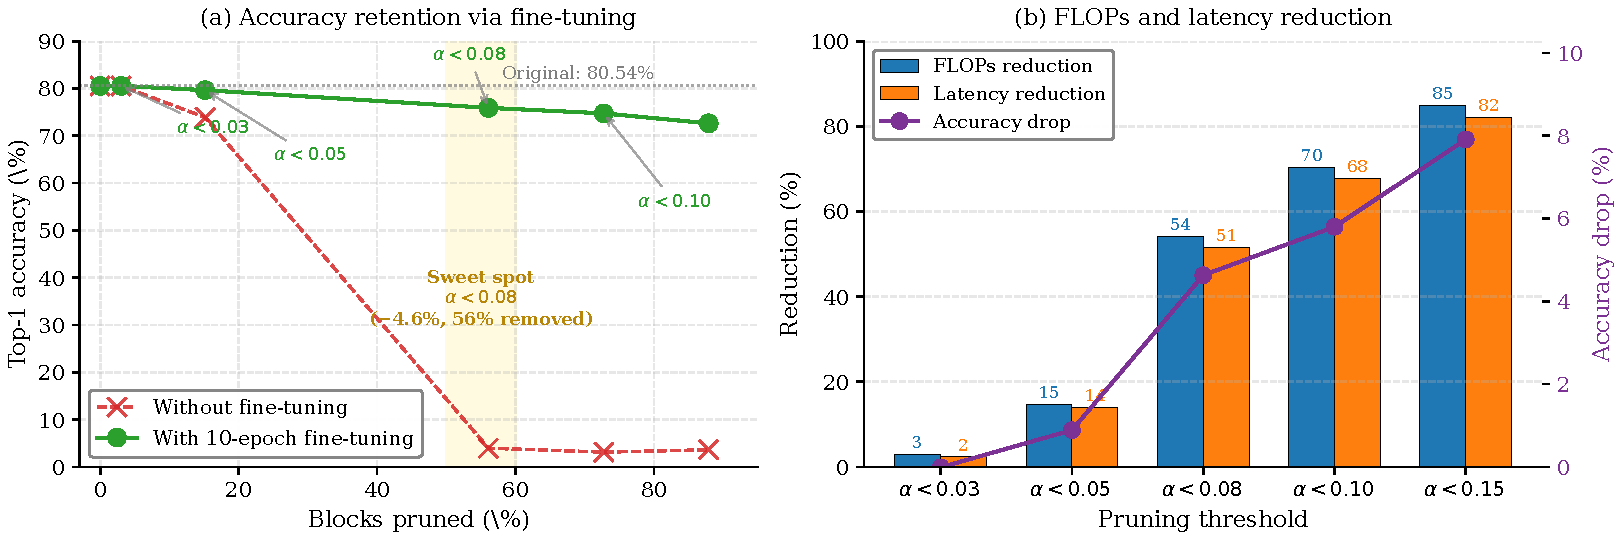
\includegraphics[width=\linewidth]{figures/fig_pruning_efficiency.pdf}
    \caption{$\alpha$-guided pruning on ResNet-200/CIFAR-100. (a) Fine-tuning recovers accuracy across all thresholds; the sweet spot is $\alpha < 0.08$ at 4.6\% drop. (b) Pruning $\alpha < 0.08$ removes 56\% of FLOPs and 51\% of inference latency, demonstrating that self-selected low-$\alpha$ blocks are functionally near-identity.}
    \label{fig:pruning}
\end{figure}

\subsection{Comparison with Existing Methods}
\label{sec:comparison_methods}

We compare LRS with residual scaling baselines at depth 152 on CIFAR-100 (Table~\ref{tab:method_comparison}, 3-seed mean). All methods fall within a $0.84\%$ band. Performance similarity is expected---this is not a method paper. LRS distinguishes itself in providing per-block interpretability (Table~\ref{tab:comparison}) at no accuracy cost.

\begin{table}[t]
\centering
\small
\caption{Residual scaling methods at depth 152, CIFAR-100 (3-seed mean). Methods perform similarly; LRS uniquely provides per-block measurement.}
\label{tab:method_comparison}
\begin{tabular}{lc}
\toprule
\textbf{Method} & \textbf{Accuracy (\%)} \\
\midrule
LayerScale & \textbf{80.56} \\
Baseline & 80.42 \\
LRS Low & 80.28 \\
Fixup & 79.79 \\
SkipInit / ReZero & 79.72 \\
\bottomrule
\end{tabular}
\end{table}

%-------------------------------------------------------------------------
\section{Discussion}
\label{sec:discussion}

\subsection{ResNets Self-Select Their Depth}

The central finding is that deep ResNets do not use their full depth. A 200-layer network concentrates transformations in 5--6 blocks---primarily at stage boundaries---and reduces the remaining 60 to near-identity. This is not an artifact of LRS measurement: identity initialization yields the same result, and pruning validation confirms that $\alpha < 0.03$ blocks truly contribute nothing.

The conventional view is that skip connections solve the degradation problem by enabling gradient flow through deep networks. Our gradient analysis (Figure~\ref{fig:gradient_flow}) confirms gradient stabilization. However, LRS reveals that the network uses this stability \emph{not} to leverage deep computation but to \emph{bypass} most blocks. The reframing: degradation is not a problem to be solved but a natural consequence of the network selecting its optimal depth. Skip connections provide the \emph{mechanism} for this self-selection by enabling blocks to act as near-identity without disrupting gradient flow.

This resonates with the unrolled-iterative-estimation view~\cite{greff2017highway} and the path ensemble interpretation~\cite{veit2016residual}. Our contribution is to make self-selection directly observable through $\alpha$ rather than inferring it from paths or lesions.

\textbf{Relation to Stochastic Depth.} Stochastic Depth~\cite{huang2016deep} demonstrates that random per-iteration block dropping during training preserves accuracy. Our finding is the converse and complementary: given a continuous knob, the network itself converges to a \emph{deterministic} near-identity for the same blocks that Stochastic Depth could randomly drop without harm. The two measure the same phenomenon---within-stage redundancy---from opposite directions (input-side noise vs.\ learned weight), and their agreement is mutual evidence. The distributed redundancy we observe under fine-tuning recovery (Section~\ref{sec:pruning}) is precisely what makes random dropping viable: blocks are not individually irreplaceable, but the network collectively allocates active roles to a small subset under standard training.

\subsection{The Role of Downsampling Blocks}
\label{sec:downsampling_role}

Per-block analysis shows that downsampling blocks maintain high $\alpha$ (0.42--0.96), while within-stage blocks converge to $\alpha < 0.15$. This grounds a design principle implicit in many efficient architectures: \emph{the number of stages (and thus downsampling operations) matters more than the total number of blocks per stage}. Three lines of prior work converge with this. MobileNet~\cite{howard2017mobilenets} and EfficientNet~\cite{tan2019efficientnet} achieve strong accuracy with shallow per-stage block counts. Stochastic Depth~\cite{huang2016deep} found dropping within-stage blocks hurts less than dropping stage-transition blocks. NAS literature~\cite{tan2019efficientnet} consistently allocates more channels at stage transitions than additional within-stage layers. LRS explains \emph{why}: the within-stage blocks these methods de-emphasize are precisely the blocks our $\alpha$ measurements flag as near-identity.

\subsection{Why Standard ResNet Still Works Well}

If the optimal $\alpha$ is much less than 0.5, why does standard ResNet (implicit $\alpha = 0.5$ in the LRS view) perform well? The answer: standard ResNet uses $y = F(x) + x$, which does not constrain the relative scale of $F(x)$ and $x$. Through batch normalization and weight magnitude adjustment, the network can effectively achieve a small $\|F(x)\|/\|x\|$ ratio without an explicit $\alpha$. LRS makes this implicit ratio observable. De \& Smith~\cite{de2020batch} independently showed that batch normalization biases residual blocks toward small $F(x)$, effectively implementing identity preference without learnable scaling. LRS confirms and quantifies this phenomenon.

\subsection{Practical Implications}
\label{sec:practical_implications}

Our findings translate into three actionable guidelines.

\textbf{(1) $\alpha$-guided structural pruning.} The strongest practical use of LRS is as an automatic block-importance criterion. Unlike magnitude-based pruning or sensitivity analysis, $\alpha$ is produced as a byproduct of training---no additional importance scoring required. The procedure is one-shot: train once with LRS, threshold $\alpha$, fine-tune for $\sim$10 epochs. We demonstrated $54\%$ FLOPs / $52\%$ latency reduction at $4.6\%$ accuracy cost (Section~\ref{sec:pruning}).

\textbf{(2) Identity-favoring initialization is essential.} The catastrophic failure of LRS High at depth 200 demonstrates that residual-favoring initialization is not merely suboptimal but actively destabilizes training. Initializing $\alpha_0 \leq 0.12$ (equivalently $\theta_0 \leq -2$) is safe across all depths we tested. This aligns with ReZero ($\alpha_0 = 0$) and SkipInit but is more permissive: $\alpha_0 \approx 0.12$ allows refinement from a non-degenerate starting point.

\textbf{(3) Architecture search.} The heterogeneous $\alpha$ distribution provides a falsifiable design heuristic: allocate capacity at stage boundaries rather than within stages. NAS procedures could use $\alpha$-statistics as a regularizer against over-deep within-stage configurations.

\subsection{Limitations}

\textbf{Scale of ImageNet evaluation.} We verify the scaling law at ImageNet depths 50 and 101 with a single seed due to compute budget; deeper ImageNet models (152, 200) and additional seeds would strengthen the claim. The CIFAR cross-seed variance of $\bar{\alpha}$ ($<1\%$ of the mean at all depths, Section~\ref{sec:alpha_convergence}) provides the relevant noise floor: the ImageNet--CIFAR gaps we observe (20--80$\times$ this noise) are too large to be seed accidents, but the absence of ImageNet-internal seed replicates means we cannot directly characterize ImageNet's own noise.

\textbf{Measurement-induced bias.} LRS adds one parameter per block and modifies the optimization landscape. The identity-initialization experiments (Section~\ref{sec:identity_init}) show convergent $\bar{\alpha}$ regardless of starting point, arguing the convergence target is intrinsic. Prior work~\cite{de2020batch} independently established that batch normalization biases standard ResNet toward identity---a phenomenon LRS makes explicit but does not create.

\textbf{Architecture scope.} The analysis is restricted to bottleneck ResNets. Basic blocks, Vision Transformers, and other residual architectures are not covered. LayerScale~\cite{touvron2021going} serves a similar stabilization role in ViTs but its per-channel parameterization does not yield the per-block scalar interpretation LRS provides.

\textbf{Threshold dependency.} The ``active block'' threshold $\alpha > 0.3$ is arbitrary. We address this by reporting (i) results across four thresholds (consistent qualitative pattern) and (ii) a threshold-free metric $D_\text{eff} = \sum_i \alpha_i$ recovering the same conclusion.

%-------------------------------------------------------------------------
\section{Conclusion}
\label{sec:conclusion}

We proposed and empirically supported a concrete answer to why deep ResNets train successfully: they autonomously select an effective depth far smaller than their nominal depth, and skip connections provide the architectural freedom that makes this self-selection possible. The thesis rests on three lines of measurable evidence.

\textbf{Self-selection happens, and it is large.} Across $120$ CIFAR runs (3 seeds, 4 depths, 2 datasets) and ImageNet at depths 50/101, deep ResNets compress effective depth to roughly $8\%$ of nominal. The depth--$\bar{\alpha}$ scaling law is consistent across datasets.

\textbf{Skip connections are the enabling mechanism.} Without them, gradients explode and training is impossible---the network has no opportunity to self-select. With them, the same depth becomes trainable specifically because the network can route information through identity.

\textbf{The selection is intrinsic, not artifact.} Random and identity initialization converge to nearly identical $\bar{\alpha}$. $\alpha$-guided pruning validates the measurement: $\alpha < 0.03$ blocks can be removed with zero accuracy loss; pruning $56\%$ of blocks yields $54\%$ FLOPs / $52\%$ latency reduction at $4.6\%$ accuracy cost.

The conventional view casts deep networks as ``working'' only when each added layer contributes positively. Our results suggest a different reading: deep networks work when they are allowed not to use most layers. Capacity not used is not wasted---it is reserve, and skip connections are the architectural mechanism that makes reserve a viable design choice.

%-------------------------------------------------------------------------
\bibliography{refs}

\end{document}
